%!TEX root = ../hr-paper.tex
\newpage
\section{Results} % (fold)
\label{sec:results}

This section will show the direct results of the intersection over union from the segmentation system. It will also show some cases where the segmentation seemed to have failed and where it succeeded.


\begin{minipage}{\linewidth}
\flushleft
\captionof{table}{IoU Results} \label{tab:results:iou} 
\begin{tabular}{ c c c c c c c c c c}
\hline
\hline
0.1		&	0.2		&	0.3		&	0.4		&	0.5		&	0.6		&	0.7		&	0.8		&	0.9		&	1		\\
0.988	&	0.973	&	0.948	&	0.905	&	0.841	&	0.769	&	0.704	&	0.631	&	0.532	&	0.117	\\
\hline
\end{tabular}\par
\bigskip
The results from the segmented characters with the labeled data from the dataset.
\end{minipage}


%2comps

\begin{figure}[ht]
  \centering
  \begin{subfigure}{0.49\textwidth}
    \centering
    \fbox{
\includegraphics[width=0.5\textwidth]{./images/results/2-comps-merged.png}}
    \caption{2 connected compoments merged}
    \label{fig:results:2cm:s}
  \end{subfigure}
  \begin{subfigure}{0.49\textwidth}
    \centering
    \fbox{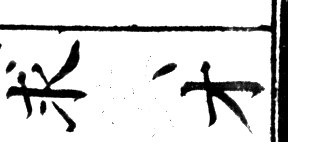
\includegraphics[width=0.5\textwidth]{./images/results/2-comps-merged-o.png}}
    \caption{Cropped image from the dataset with the original character}
    \label{fig:results:2cm:o}
  \end{subfigure}
  \caption{The merger of two connected components illustrated}
  \label{fig:results:2cm}
\end{figure}


%small image

\begin{figure}[ht]
  \centering
  \begin{subfigure}{0.49\textwidth}
    \centering
    \fbox{
\includegraphics[width=0.05\textwidth]{./images/results/small-whitespace.png}}
    \caption{A small character segmented correctly}
    \label{fig:results:sw:s}
  \end{subfigure}
  \begin{subfigure}{0.49\textwidth}
    \centering
    \fbox{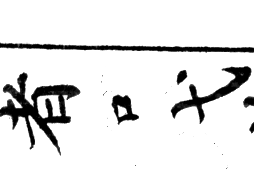
\includegraphics[width=0.5\textwidth]{./images/results/small-whitespace-o.png}}
    \caption{Cropped image from the dataset with the original character}
    \label{fig:results:sw:o}
  \end{subfigure}
  \caption{original character and segmented character next to each other}
  \label{fig:results:sw}
\end{figure}

%2 in one

\begin{figure}[ht]
  \centering
  \fbox{
\includegraphics[width=0.25\textwidth]{./images/results/2inone.png}}
  \caption{Two characters segmented as one}
  \label{fig:results:2i1}
\end{figure}

\newpage

%3 lines

\begin{figure}[ht]
  \centering
  \begin{subfigure}{0.49\textwidth}
    \centering
    \fbox{
\includegraphics[width=0.01\textwidth]{./images/results/3-lines.png}}
    \caption{Character partially removed}
    \label{fig:results:3l:s}
  \end{subfigure}
  \begin{subfigure}{0.49\textwidth}
    \centering
    \fbox{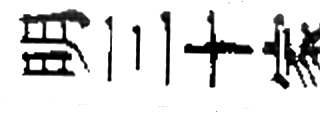
\includegraphics[width=0.5\textwidth]{./images/results/3-lines-o.png}}
    \caption{Cropped image from the dataset with the original character}
    \label{fig:results:3l:o}
  \end{subfigure}
  \caption{Character in the dataset and the segmented character}
  \label{fig:results:3l}
\end{figure}

%1.5

\begin{figure}[ht]
  \centering
  \begin{subfigure}{0.49\textwidth}
    \centering
    \fbox{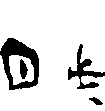
\includegraphics[width=0.3\textwidth]{./images/results/15-1.png}}
    \caption{First character split}
    \label{fig:results:15:s1}
  \end{subfigure}
  \begin{subfigure}{0.49\textwidth}
    \centering
    \fbox{
\includegraphics[width=0.3\textwidth]{./images/results/15-2.png}}
    \caption{Second character split}
    \label{fig:results:15:s2}
  \end{subfigure}
    \begin{subfigure}{\textwidth}
    \centering
    \fbox{
\includegraphics[width=0.6\textwidth]{./images/results/15-o.png}}
    \caption{Cropped image from the dataset with the original character}
    \label{fig:results:15:o}
  \end{subfigure}
  \caption{Character Split wrongly to contain 1.5 of character}
  \label{fig:results:15}
\end{figure}

\newpage

%Big line

\begin{figure}[ht]
  \centering
  \fbox{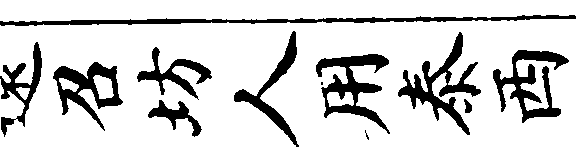
\includegraphics[width=0.8\textwidth]{./images/results/big-line.png}}
  \caption{Character segmentation with a noise line}
  \label{fig:results:bl}
\end{figure}


%Blackbar

%Noise ball

\begin{figure}[ht]
  \centering
  \begin{subfigure}{0.49\textwidth}
    \centering
    \fbox{
\includegraphics[width=0.05\textwidth]{./images/results/noise-ball.png}}
    \caption{`Noise ball'}
    \label{fig:results:noise:nb}
  \end{subfigure}
  \begin{subfigure}{0.49\textwidth}
    \centering
    \fbox{
\includegraphics[width=0.05\textwidth]{./images/results/blackbar.png}}
    \caption{`Black bar'}
    \label{fig:results:noise:bb}
  \end{subfigure}
  \caption{Character segmentation of noise components}
  \label{fig:results:noise}
\end{figure}





% - image to big due to line noise
% image to big due to other noise
% correct small
% 2 in one
% - 1.5

% section results (end)
